\chapter{Análisis Exploratorio de Datos} \cite{LSBM} \cite{PHPDAT}

El análisis exploratorio de datos o EDA de sus siglas en inglés “Exploratory Data Analysis” es un procedimiento estadístico que sirve de herramienta para el tratamiento de datos con el fin de encontrar relaciones en los datos obtenidos en diferentes tipos de estudios. 

\bigskip

De metodología relativamente sencilla y sistemática puede organizar los datos para encontrar conjuntos con relaciones fuertes entre sus observaciones (clusters), observaciones que se encuentran fuera de esas relaciones (outliers) y mediante el estudio de estas últimas comprobar si están fuera de esos rangos por errores en las mediciones o por ser casos especiales de estudio.

\bigskip

EDA trata de hacer un análisis cualitativo de los datos para poder extraer información relevante de los mismos. En primer lugar se organizan los datos para el estudio mediante una estandarización de las variables de manera que podamos aplicar las técnicas estadísticas para conseguir la media, varianza, covarianza y demás modelos multivariantes del conjunto a estudiar. A continuación se realiza una visualización de las relaciones existentes. Y por último estudiar los patrones “especiales” como los outliers para ver porqué lo son y si nos son de utilidad en la investigación.

\bigskip

En el siguiente apartado se expondrán las técnicas de proyección de EDA que se van a utilizar en este trabajo.

\bigskip

\section{Técnicas de proyección}
Dentro de todas las posibles técnicas a utilizar para el análisis exploratorio de datos, en este proyecto se van a desarrollar dos principalmente y luego se comentarán algunas de las herramientas mediante las cuales se aplicarán dichas técnicas.
\bigskip 

Las técnicas a utilizar son el análisis de componentes principales o \textbf{PCA} “Principal Component Analysis” y mínimos cuadrados parciales o \textbf{PLS} “Parcial Least Squares”. Por otra parte también existen muchas técnicas gráficas para representar de manera visual los conjuntos de datos como son los gráficos “Score Plots”, “Loading Plots”, MEDA, oMEDA, etc.
\bigskip

Tanto PCA como PLS tratan el mismo problema de la colinealidad de los datos pero en casos diferentes.
\bigskip

Mientras que PCA es mas útil en problemas no supervisados PLS se emplea para los supervisados.
\bigskip
 
Los problemas supervisados son en los que se dispone de información de clases, estando los datos categorizados y haciendo posible el establecimiento de un modelo que ayude a la obtención de resultados en futuros análisis.
\bigskip

Los problemas no supervisados son para los que no hay un propósito específico, no se han seleccionado un conjunto de muestras, ni de variables con las que relacionarlas. Se trabaja sobre un conjunto de datos obtenido sin supervisión y sólo se puede llevar a cabo un análisis para encontrar tendencias o patrones en los mismos, para clasificarlos.
\bigskip

Ambos métodos (PCA y PLS)se basan en la utilización de variables latentes o LVs. Estas variables en PCA se llaman componentes principales o PC y se infieren a partir de la varianza de los datos. En el caso de PLS las se obtienen de la covarianza. 
\bigskip

La reducción del tamaño es esencial cuando tratamos con “Big Data”, donde  cualquier disminución del tamaño del problema agiliza el trabajo, por ello estas técnicas son de gran importancia para el propósito de este proyecto.
\bigskip


\section{Análisis de componentes principales PCA} \cite{EKE} \cite{JMMD}

En este tipo de análisis se utilizan los PCs como se ha comentado en el apartado anterior, los cuales nos ayudan a reducir el tamaño del problema puesto que al inferirlos se eliminan los datos redundantes o repetidos. 
\bigskip

Estas nuevas variables obtenidas son combinaciones lineales de las variables del conjunto de datos inicial. Lo que se pretende con esto es que de un conjunto inicial M  obtener un conjunto A siendo $ A \leq M $. En el caso que M y A fueran iguales el proceso de obtención de las componentes principales no ha reducido el tamaño del problema, lo cual quiere decir que no existe redundancia en los datos ni repetición de los mismos.
\bigskip

En PCA tenemos una matriz, llamémosla X, de tamaño NxM donde las columnas son las variables del estudio y las filas o tuplas son muestras de la población a estudiar u observaciones. La forma de dicha matriz sería X = estructura + residuo, siendo más concretos 

%
\begin{equation}
X= T_A*P_A’ + E_A
\end{equation} 

Donde $T_A$ es la matriz de puntuaciones, que almacena las proyecciones de las observaciones en los PCs, $P_A$ es la matriz de cargas con los autovectores del producto cruzado $X'*X$, $E_A$ es la matriz de residuos, y A es el número de PCs. 
\bigskip

\begin{figure}[H]
\centering
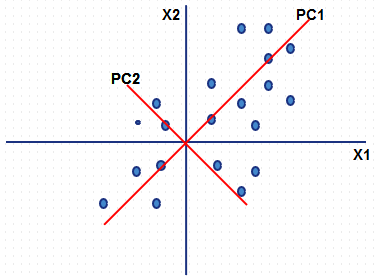
\includegraphics[width=0.9\textwidth]{imagenes/figuras/2_1.png}
\caption{Descripción gráfica de componente principal.}
\end{figure}

Los componentes principales se pueden calcular como combinaciones lineales de las variables originales minizando la suma de cuadrados de las distancias de cada punto al subespacio, maximizando la variabilidad o con regresiones alternas.
\bigskip

Previamente al cálculo de las componentes principales se hace el “centrado de datos” mediante el cual, calculada la media de los valores, se trasladan los ejes de coordenadas a ese punto intermedio, esto se hace restando a cada punto el valor de la media del conjunto, quedando el valor medio en el origen. El número de ejes ortogonales entre sí dependerá del número de componentes principales que se calculen.

\bigskip

En la figura 2.1 se puede ver gráficamente esto, aunque en este caso la dimensión no varía se aprecia como se han representado todo los puntos mediante PC1 y PC2.

\bigskip

Una vez realizada la selección de las variables latentes se pasaría a estudiar las relaciones entre observaciones mediante gráficos como los que se comentarán en los siguientes apartados.
\bigskip


\section{Mínimos cuadrados parciales PLS}
Esta técnica de proyección de datos se da en entornos supervisados, es decir, cuando se dispone de una o varias variables respuesta que guían la exploración. A diferencia del caso anterior las variables latentes que este modelo utiliza se obtienen de la covarianza entre X e Y. El modelo tiene como estructura:

\begin{equation}
X= T_A*P_A^T+E_A
\end{equation}

\begin{equation}
Y= T_A*Q_A^T+F_A
\end{equation}

Donde \textbf{$P_A$}  y \textbf{$Q_A$} son las matrices de carga de tamaño \textbf{A} (número de variables latentes), \textbf{$T_A$} son las matrices de puntuaciones y \textbf{$E_A$} y \textbf{$F_A$} son las de residuos.
\bigskip
También se puede obtener la matriz Y a partir de la X mediante la siguiente función:
\begin{equation}
Y=X*B_A+F_A
\end{equation}


Donde la matriz \textbf{$B_A$} añade los coeficientes de regresión.

\bigskip
Dentro de este método existe una variante  llamada “Mínimos cuadrados parciales – Análisis discriminante” en el que la matriz Y se genera artificialmente con variables “dummy”, una por cada clase del conjunto de datos original. La pertenencia de una variable a una clase se identifica dándole valor uno a la clase que pertenezca y -1 al resto.

\bigskip

\section{Análisis Exploratorio de Datos Multivariante}
\subsection{MEDA}
Dentro de las herramientas del análisis exploratorio de datos se encuentra \textbf{MEDA}, que es una técnica basada en la comparación de variables de forma múltiple. No se basa en el análisis individual de cada una de las variables del conjunto por separado si no en una visión global de las mismas estudiando sus relaciones y cómo de correladas se encuentran entre sí.
\bigskip

En el caso que ocupa este proyecto estudiaremos las formas de visualizar dichas relaciones mediante distintos tipos de gráficos que nos mostraran a simple vista los vínculos, si existen, entre variables
\bigskip

La matriz MEDA que se genera es de tamaño \textbf{MxM}, siendo \textbf{M} el número de variables. En cada una de las celdas de \textbf{M} se almacenará un valor entre -1 y 1 que corresponde a la relación que existe entre la variable i y la j, creándose así una estructura con todas las relaciones posibles. Esta relación se calcula cómo: 
\begin{equation}
q^2_{A,(m,l)}=1-\frac{\parallel \widehat{e}_{A,(l)}\parallel ^2}{\parallel x_{(l)} \parallel ^2} ,\forall l \neq m
\end{equation}


Donde \textbf{$q_{A,(m,l)}$} es cada uno de los valores de la matriz MEDA, \textbf{$\widehat{e}_{A,(l)}$} corresponde a cada uno de los errores en la estimación de la variable \textbf{l} y \textbf{$x_{(l)}$}  es el valor de la variable en análisis. De esta ecuación podemos entender el funcionamiento de MEDA de forma rápida ya que lo que aquí se expresa es que cada uno de los valores de la matriz MEDA será más próximo a cero cuanto mayor sea el error y más próximo a 1 o -1 cuanto mejor sea la estimación.
\bigskip

Utilizando MEDA junto con los modelos de proyección anteriores (PLS y PCA) podremos comprender mejor las relaciones entre variables, ya que mientras que las técnicas de proyección vistas reducen el tamaño del problema y eliminan la colinealidad de los datos, MEDA se encarga de la correlación entre variables.
\bigskip

Con los gráficos MEDA podemos observar mediante un “código de colores” lo relacionadas que están las variables entre sí. Como los valores de la matriz MEDA van desde el -1 hasta el 1 los colores van desde el azul que representa al -1 al rojo que representa al 1, el cero es representado por el blanco y cada valor entre dichos rangos tendrá un color degradado dentro de los mismos. Si el valor se acerca a cero por debajo, es decir -0.1 por ejemplo el color que se verá en el gráfico es un azul muy claro, mientras que si es por arriba, como el 0.1 se verá de un rojo difuminado casi blanco.
\bigskip

\begin{figure}[H]
\centering
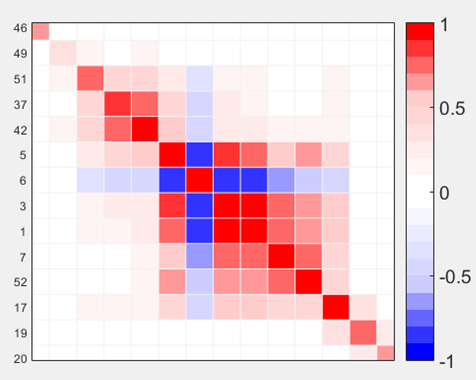
\includegraphics[width=0.9\textwidth]{imagenes/figuras/2_3.png}
\caption{Ejemplo de gráfico MEDA.}
\end{figure}

La figura 2.2 muestra un ejemplo de gráfico MEDA,  ampliado para que sólo se muestre una parte del mismo, de esta forma se pueden apreciar los distintos degradados de color escalados por los colores de la derecha de la imagen. Se puede ver como la variable 5 y la 6 tienen una fuerte relación pero inversa, mientras que la 5 con la 3 tienen una fuerte relación directa.

\bigskip

\subsection{oMEDA}

Este método derivado del anterior se encarga de relacionar variables con observaciones para ver cuáles de ellas (variables) están más relacionadas con patrones descritos en las observaciones.
\bigskip

Este método aplica MEDA sobre los datos originales con una variable que represente las observaciones de interés, incluyéndola en el conjunto de variables mediante un vector columna que da valores a cada observación dividiendo el conjunto en grupos de observaciones a comparar.
\bigskip

Éste método da valores de 1, 0 y -1 en dicho vector de observaciones siendo 1 las observaciones a estudiar, -1 a los datos con los que se quiere comparar dichas observaciones y 0 a todas las que no se quieren estudiar, ignorando por tanto oMEDA todas las variables que tengan dicho 0.
\bigskip

\begin{figure}[H]
\centering
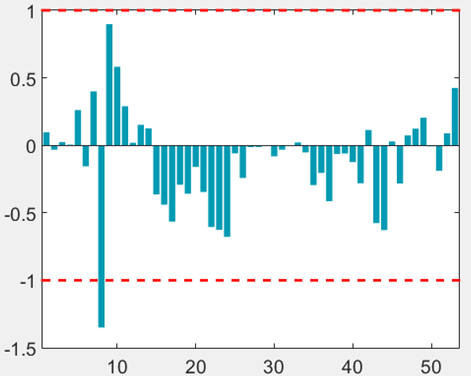
\includegraphics[width=0.9\textwidth]{imagenes/figuras/2_4.png}
\caption{Ejemplo de oMEDA.}
\end{figure}

\bigskip

En la figura 2.3 se tiene un ejemplo de oMEDA, en el que se puede apreciar como dentro del conjunto de observaciones seleccionado la variable 8 y la 9 son las que mas importancia toman en la relación.

\subsection{Score Plots}

Este tipo de gráficos se utilizan para ver de forma rápida la distribución de las observaciones en el sub-espacio de variables latentes por parejas de las mismas. 
\bigskip

En un eje de coordenadas se sitúa una variable y en el otro otra, elegidas por el analista, y así podemos observar la existencia de clusters, outliers o cualquier tipo de patrón en los datos que nos dé una idea de qué relación existe entre las observaciones. Con este método podemos ver las diferencias existentes entre conjuntos de datos que pueden tener modelos PCA o PLS iguales. Se utiliza para interpretar las relaciones entre las observaciones.

\begin{figure}[H]
\centering
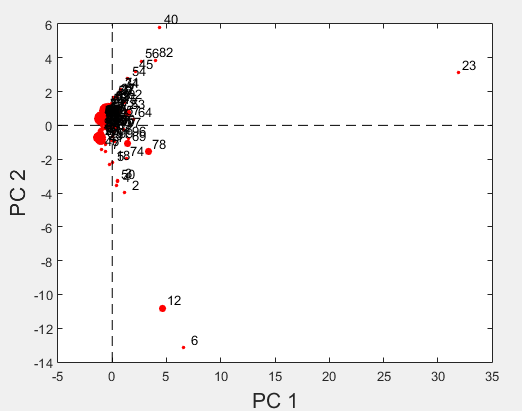
\includegraphics[width=0.9\textwidth]{imagenes/figuras/2_5.png}
\caption{Ejemplo de Score Plot.}
\end{figure}
\bigskip

En la figura 2.4 se pueden observar varios elementos notables, mientras que en el origen de coordenadas se puede ver un cluster, tambien se observan 3 outliers identificados por las etiquetas 23, 12 y 6.

\subsection{Loading Plots}

Similar al anterior los loading plots nos muestran la correlación entre variables. Al igual que el anterior, se seleccionan dos LVs y este gráfico nos muestra lo correladas que están entre sí, viendo si dicha correlación es positiva o negativa. Si dos registros se encuentran muy juntos entre sí podemos decir que su correlación es positiva, mientras que si mantienen una distancia “simétrica” con respecto al origen podemos decir que es negativa. La diferencia con el anterior es que en este caso se utiliza para interpretar las diferencias entre las variables y no entre las observaciones.

\begin{figure}[H]
\centering
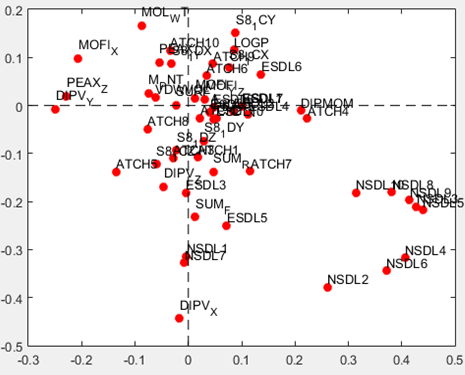
\includegraphics[width=0.9\textwidth]{imagenes/figuras/2_6.png}
\caption{Ejemplo de Loading Plot.}
\end{figure}

En el caso de la figura 2.5 no se pueden apreciar tendencias o patrones en las variables ya que es complicado identificar clusters  u outliers en la visualización.